\documentclass[12pt]{beamer}

\usepackage{pgfpages} %This is needed for notes presentation!
%\setbeameroption{}

\usepackage{enumerate, amsmath, amssymb,amsthm, amstext,color}
\usepackage[ngerman, english]{babel}
\usepackage[latin1]{inputenc}   
\usepackage{dsfont}
\usepackage{geometry}
\usepackage{fancyhdr}
\usepackage{tikz}
\usetikzlibrary{plotmarks}
\usetikzlibrary{arrows, positioning}
\usepackage{lmodern}
\usepackage{textcomp}
\usepackage{textpos}
\usepackage{relsize}


\usepackage{float}
\usepackage{color}
\usepackage{hyperref}
% \usepackage{algorithmicx}
% \usepackage{algpseudocode}
\usepackage{fancybox}
\usepackage{float}
\usepackage{sidecap}


%\setbeamertamplate[circle]



\newcommand{\lk}{\left}
\newcommand{\rk}{\right}
\newcommand{\rel}{\sqsubseteq}
\newcommand{\rhn}{\mathds{R}^n}
 
\usetheme{Madrid} % Antibes, Berlin, darmstadt, default, Frankfurt; JuanLesPins
%\usetheme{
%	AnnArbor | Antibes | Bergen |
%	Berkeley | Berlin | Boadilla |
%	boxes | CambridgeUS | Copenhagen |
%	Darmstadt | default | Dresden |
%	Frankfurt | Goettingen |Hannover |
%	Ilmenau | JuanLesPins | Luebeck |
%	Madrid | Malmoe | Marburg |
%	Montpellier | PaloAlto | Pittsburgh |
%	Rochester | Singapore | Szeged |
%	Warsaw
%}
\usecolortheme{beaver}
% \usecolortheme{
% 	albatross | beaver | beetle |
% 	crane | default | dolphin |
% 	dove | fly | lily | orchid |
% 	rose |seagull | seahorse |
% 	sidebartab | structure |
% 	whale | wolverine
% }

\useinnertheme{rounded}
% \useinnertheme{
% 	circles | default | inmargin |
% 	rectangles | rounded
% }

\useoutertheme{infolines}
% \useoutertheme{
% 	default | infolines | miniframes |
% 	shadow | sidebar | smoothbars |
% 	smoothtree | split | tree
% }

\usefonttheme{default}
% \usefonttheme{
% 	default | professionalfonts | serif |
% 	structurebold | structureitalicserif |
% 	structuresmallcapsserif
% }

% Seitenzahlen
\setbeamertemplate{footline}[frame number]

\title{Real Time Control of a Quadcopter}
\author{Simon Kick, Philipp Fr\"ohlich, Benedikt K\"onig, Annika Stegie}
\institute{Technische Universit\"at M\"unchen}
\date{11 July 2015}
% \titlegraphic{\pgfimage[width=1cm,height=1cm]{MA_Web}}
%\logo{\pgfimage[width=1.2cm,height=1.2cm]{MA_Web}}

\beamertemplatenavigationsymbolsempty
% kleine Symbole zur Nvigation wegmachen

\setcounter{MaxMatrixCols}{20}

%\AtBeginSection[]
%{
%	\begin{frame}
%	\frametitle{Overview}
%	\tableofcontents[currentsection]
%	\end{frame}
%}


\begin{document}


\begin{frame}
\maketitle
\thispagestyle{empty}
\end{frame}

%\begin{frame}{Overview}
%\tableofcontents
%\end{frame}
%
% 1.  Folie mit Poster-Bild zur Erklärung was wir überhaupt machen - ok
% 2.  Mindmap mit den Bausteinen unseres Projekts
% 3.  Formulierung unseres Optimierungsproblems -> kurz warum SQP
%     Erklärung wann dikretisierung??? in Folien???
% 4.  Mindmap mit Haken bei Problem-Formulierung?
% 5.  Modell -> Bilder schön einzeln und Formeln immer mit passenden Bildern
% 6.  ?????? Lösung der ODEs mit multiple shooting Ansatz????
% 7.  Mindmap Modell abgehakt
% 8.  Realtime, Riccati, ... Zeitenvergleich mit und ohne Riccati
% 9.  Mindmap Realtime ok
% 10. Ergebnisse: Wind, verschiedene Flugbahnen, mit und ohne stabilisierung, ...


\begin{frame}
	\frametitle{Motivation}
	
	\begin{figure}[p]
		\centering
		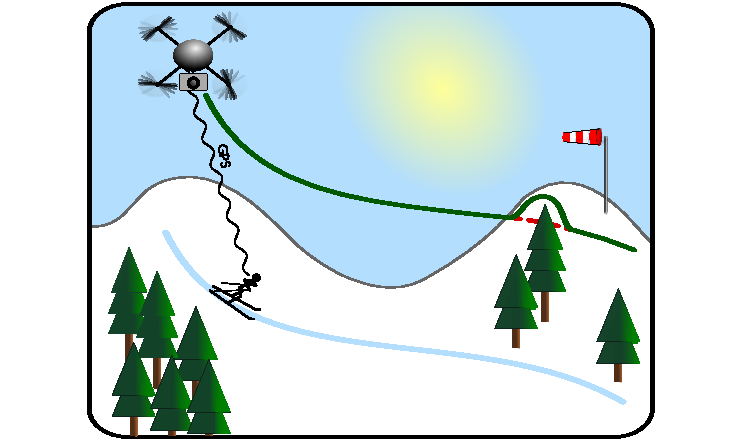
\includegraphics[width=\columnwidth]{images/Motivationsfolie}
	\end{figure}
	
\end{frame}

%\begin{frame}
	%\frametitle{Optimal Control Formulation}
	%\begin{block}{}
		%%\begin{center}
		 %%\parbox{9.5cm}{\( \min \limits_{x,u} J(x,u) \qquad  \) s.t. \parbox{\textwidth}{
				%%\( \qquad \left. \begin{array}{c} \tilde{h}(x,u)=0 \\  \dot{x} = f(x,u) \end{array} \right.\)	}}
				%%\begin{align*}
					%%x: & \quad \text{state} \\
					%%u: & \quad \text{control}
				%%\end{align*}
		%%\end{center}
		%\begin{center}
		 %\parbox{9.5cm}{\( \min \limits_{x,u} J(x,u) \quad  \) s.t. \parbox{\textwidth}{
				%\( \quad \left. \begin{array}{c} \tilde{h}(x,u)=0 \\  \dot{x}(t) = f(x(t),u(t)) \end{array} \right.\)	}}
				%\begin{align*}
					%x: & \quad \text{state} \\
					%u: & \quad \text{control}
				%\end{align*}
		%\end{center}
	%\end{block}
%\end{frame}

\begin{frame}
	\frametitle{Optimal Control Formulation}
	\begin{block}{}
		%\begin{center}
		 %\parbox{9.5cm}{\( \min \limits_{x,u} J(x,u) \qquad  \) s.t. \parbox{\textwidth}{
				%\( \qquad \left. \begin{array}{c} \tilde{h}(x,u)=0 \\  \dot{x} = f(x,u) \end{array} \right\} \Rightarrow h(x,u) = 0 \)	}}
				%\begin{align*}
					%x: & \quad \text{state} \\
					%u: & \quad \text{control}
				%\end{align*}
		%\end{center}
		\begin{center}
		 \parbox{9.5cm}{\( \min \limits_{x,u} J(x,u) \quad  \) s.t. \parbox{\textwidth}{
				\( \quad \left. \begin{array}{c} \tilde{h}(x,u)=0 \\  \dot{x}(t) = f(x(t),u(t)) \end{array} \only<1>{\right.} \only<2->{\right\} \Rightarrow h(x,u) = 0	}\)}}
				\begin{align*}
					x: & \quad \text{state} \\
					u: & \quad \text{control}
				\end{align*}
		\end{center}
	\end{block}
\end{frame}

%\begin{frame}
	%\frametitle{SQP-Formulation}
	%
	%\begin{block}{}
		%\centering
			%\parbox{7cm}{\( \min \limits_{x,u} J(x,u) \qquad \text{s.t.} \qquad h(x,u) = 0 \)	}
%\end{block}
	%
	%\uncover<2>{
		%\center{
		%reformulation as SQP-Problem \\
		%\vspace{1ex}
		%\(\Downarrow\)
		%\vspace{1em}
		%}
		%
		%
		%\begin{block}{}
		%\centering
			%\parbox{7cm}{\[ \min \limits_{s} \nabla J(x,u)^T s + \frac{1}{2}s^T \nabla^2 J(x,u)s \]
			 %\[ \text{s.t.} \quad  h(x,u) + \nabla h(x,u)^Ts = 0 \]	}
	%\end{block}
	%}
	%
%\end{frame}
\section{Model}

\begin{frame}
	\frametitle{Model}
				\begin{figure}[p]
					\centering
					\includegraphics<1>[width=11cm]{images/Copter_leer.pdf}
  				\includegraphics<2>[width=11cm]{images/Copter_Fg.pdf}
					\includegraphics<3>[width=11cm]{images/Copter_Rotorrichtung_zwei.pdf}
					\includegraphics<4>[width=11cm]{images/Copter_Rotorrichtung.pdf}
					\includegraphics<5>[width=11cm]{images/Copter_Rotorkraefte.pdf}
				\end{figure}
\end{frame}

		\begin{frame}
		\frametitle{Forces}
			\begin{columns}[T] % align columns
			\begin{column}{.6\textwidth}
				\begin{textblock}{0}(-2,-6.5)
					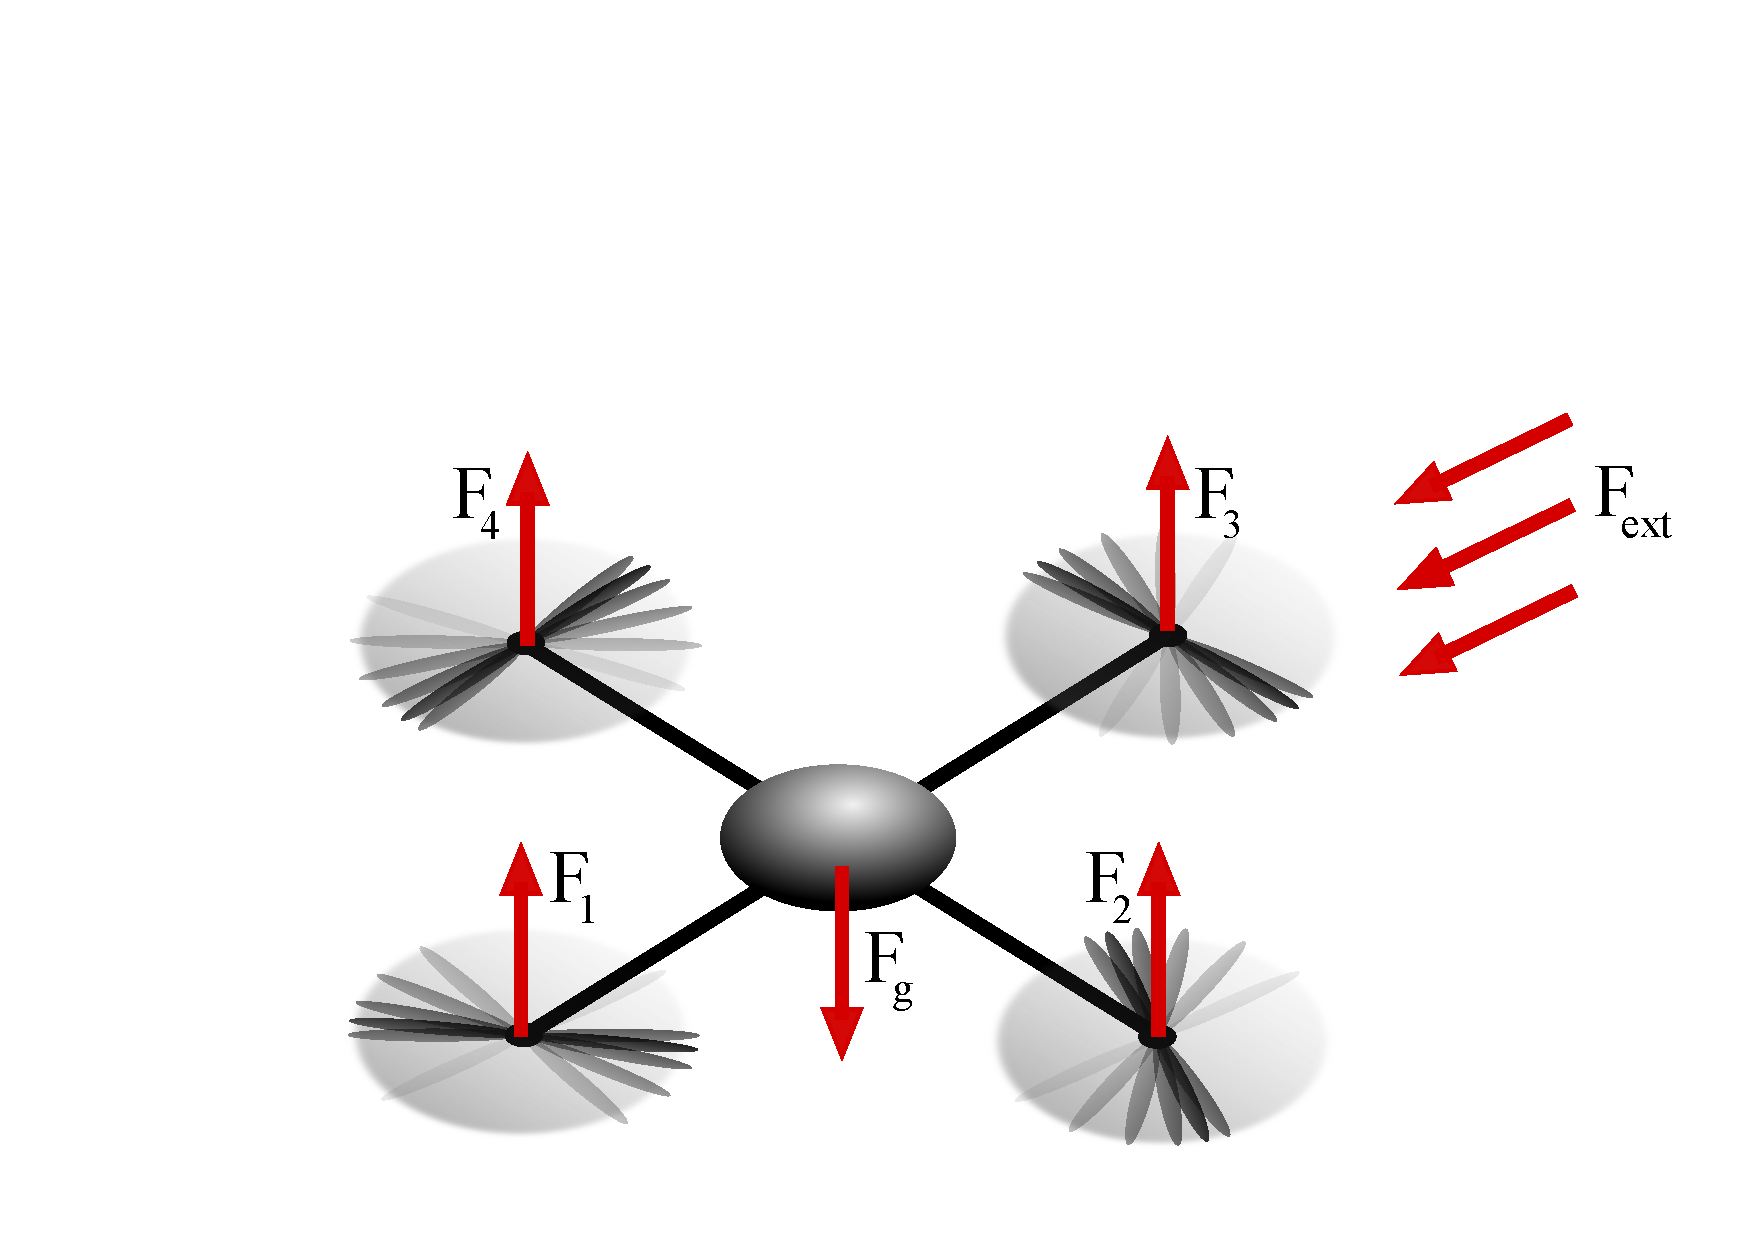
\includegraphics[width=11cm]{images/Copter_Fext_2.pdf}
				\end{textblock}
			\end{column}
			\begin{column}{0.39\textwidth}
				\begin{textblock}{0}(-.7,0.6)
					\[ \mathlarger{F_{res} =F_{ext} + F_{g} + \sum_{i=1}^{4}{F_{i}}} \]
				\end{textblock}
				\end{column}
		\end{columns}
\end{frame}

\begin{frame}
	\frametitle{Torques}
	
			\begin{figure}[p]
					\centering
					\includegraphics<1>[width=11cm]{images/Copter_axis.pdf}
				%
					%\includegraphics<2>[width=11cm]{images/Copter_psi.pdf}
%
					%\includegraphics<3>[width=11cm]{images/Copter_phi.pdf}

					\includegraphics<2>[width=11cm]{images/Copter_theta.pdf}
				\end{figure}
		
\end{frame}

\begin{frame}
		\frametitle{Torques}
			\begin{columns}[T] % align columns
			\begin{column}{.7\textwidth}
				\begin{textblock}{0}(-1,-5.3)
					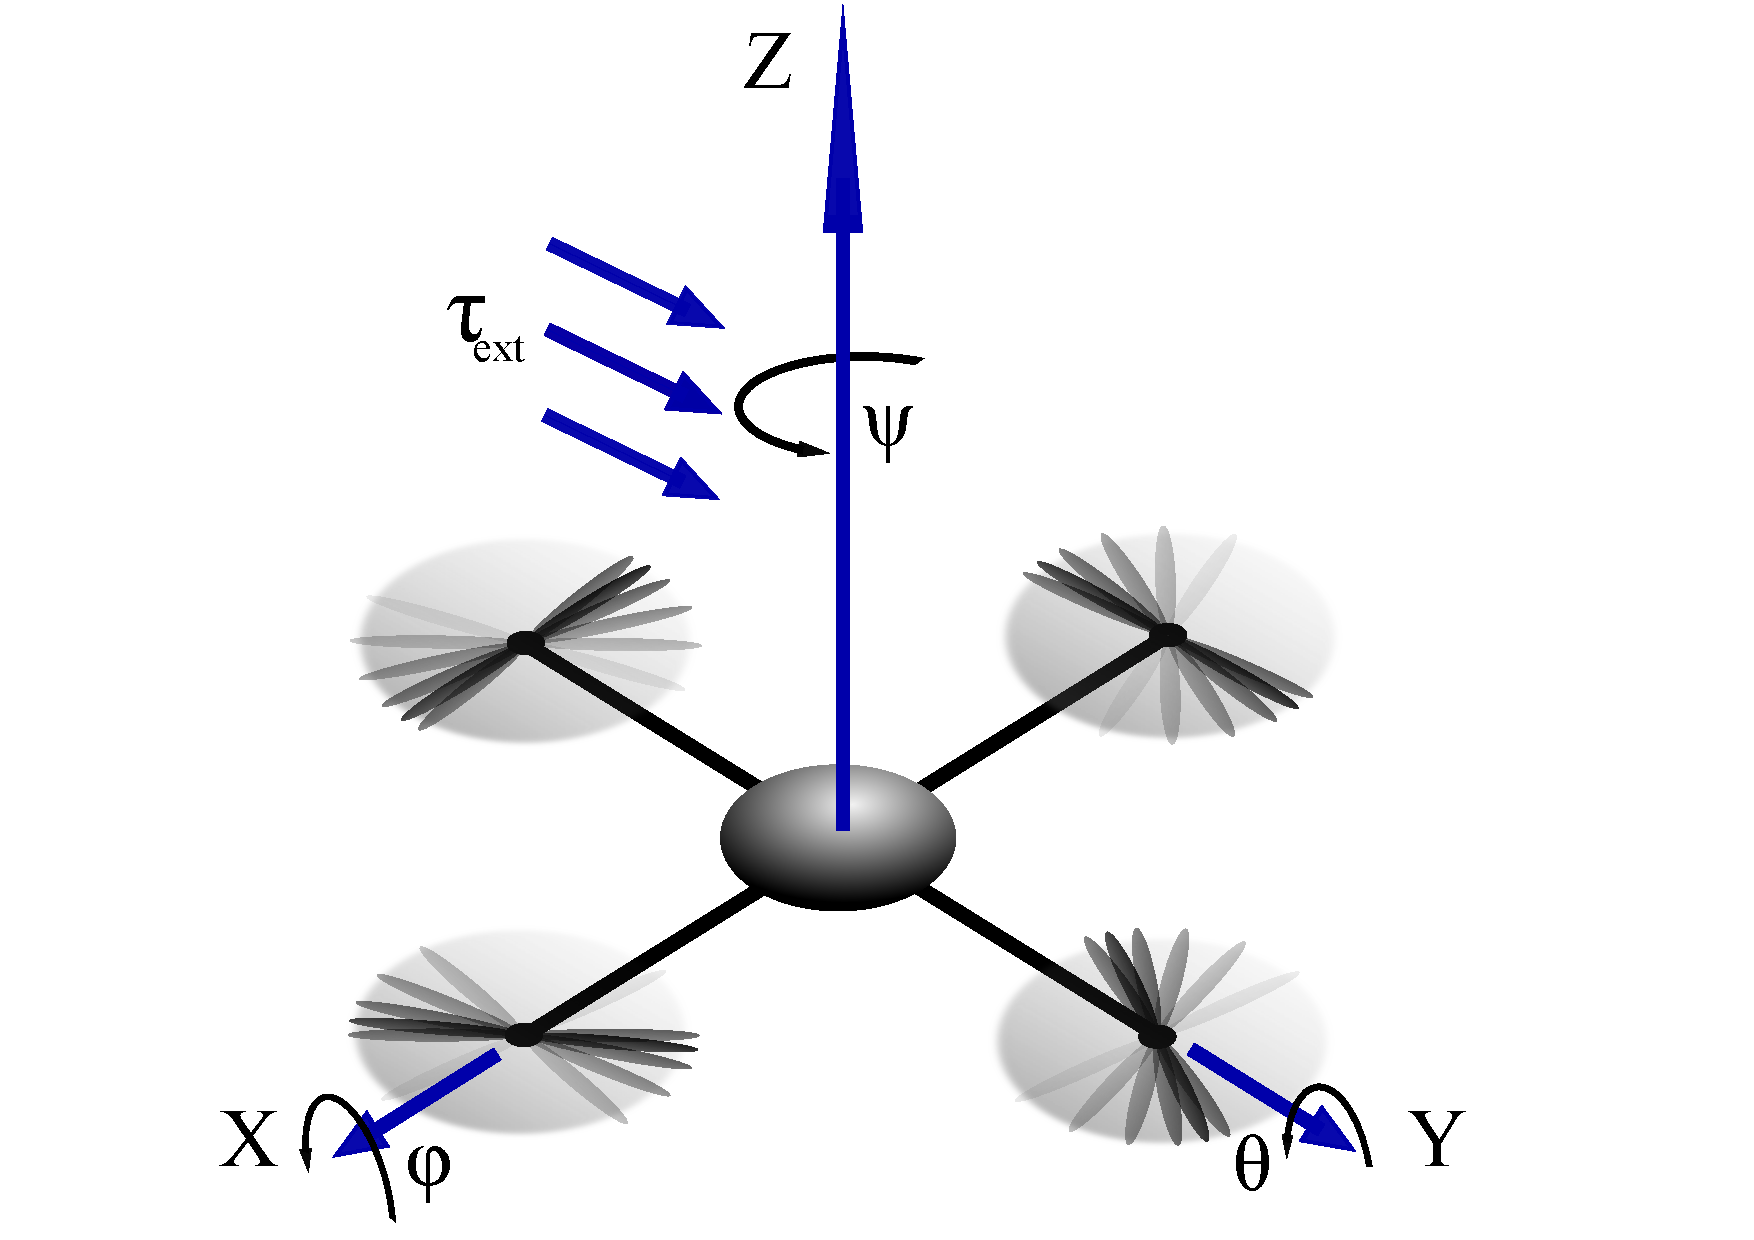
\includegraphics[width=11cm]{images/Copter_Text.pdf}
				\end{textblock}
			\end{column}
			\begin{column}{0.35\textwidth}
				\begin{textblock}{0}(-3,-3.4)
					\[ \mathlarger{\mathlarger{\tau_{res} = \tau_{ext}+\tau_{\psi}+\tau_{\varphi}+\tau_{\theta}}} \]
				\end{textblock}
				\end{column}
		\end{columns}
\end{frame}

\begin{frame}
	\frametitle{Obtain ODE}
	\begin{block}{}
		\centering
		\[\left. \begin{array}{rl} F_{res} \hspace{-1.25ex} &= F_{ext} + F_{g} + \sum_{i=1}^{4}{F_{i}} \\ \tau_{res} \hspace{-1.25ex} &= \tau_{ext} + \tau_{\psi} + \tau_{\varphi} + \tau_{\theta}  \end{array} \right\} \quad \Rightarrow \quad \dot{x}(t)=f(x(t),u(t)) \]
		\vspace{1ex}
	\end{block}
	
	\vspace{2em}
	
	\onslide<2->
	
	\begin{block}{}
		\begin{center}
		 	\[ \quad \left. \begin{array}{c} \tilde{h}(x,u)=0 \\  \dot{x}(t) = f(x(t),u(t)) \end{array} \right\} \Rightarrow h(x,u) = 0	\]
		\end{center}
		\vspace{1ex}
	\end{block}
	
\end{frame}


\begin{frame}
	\frametitle{Copter Rotation}
		\begin{figure}[p]
			\centering
			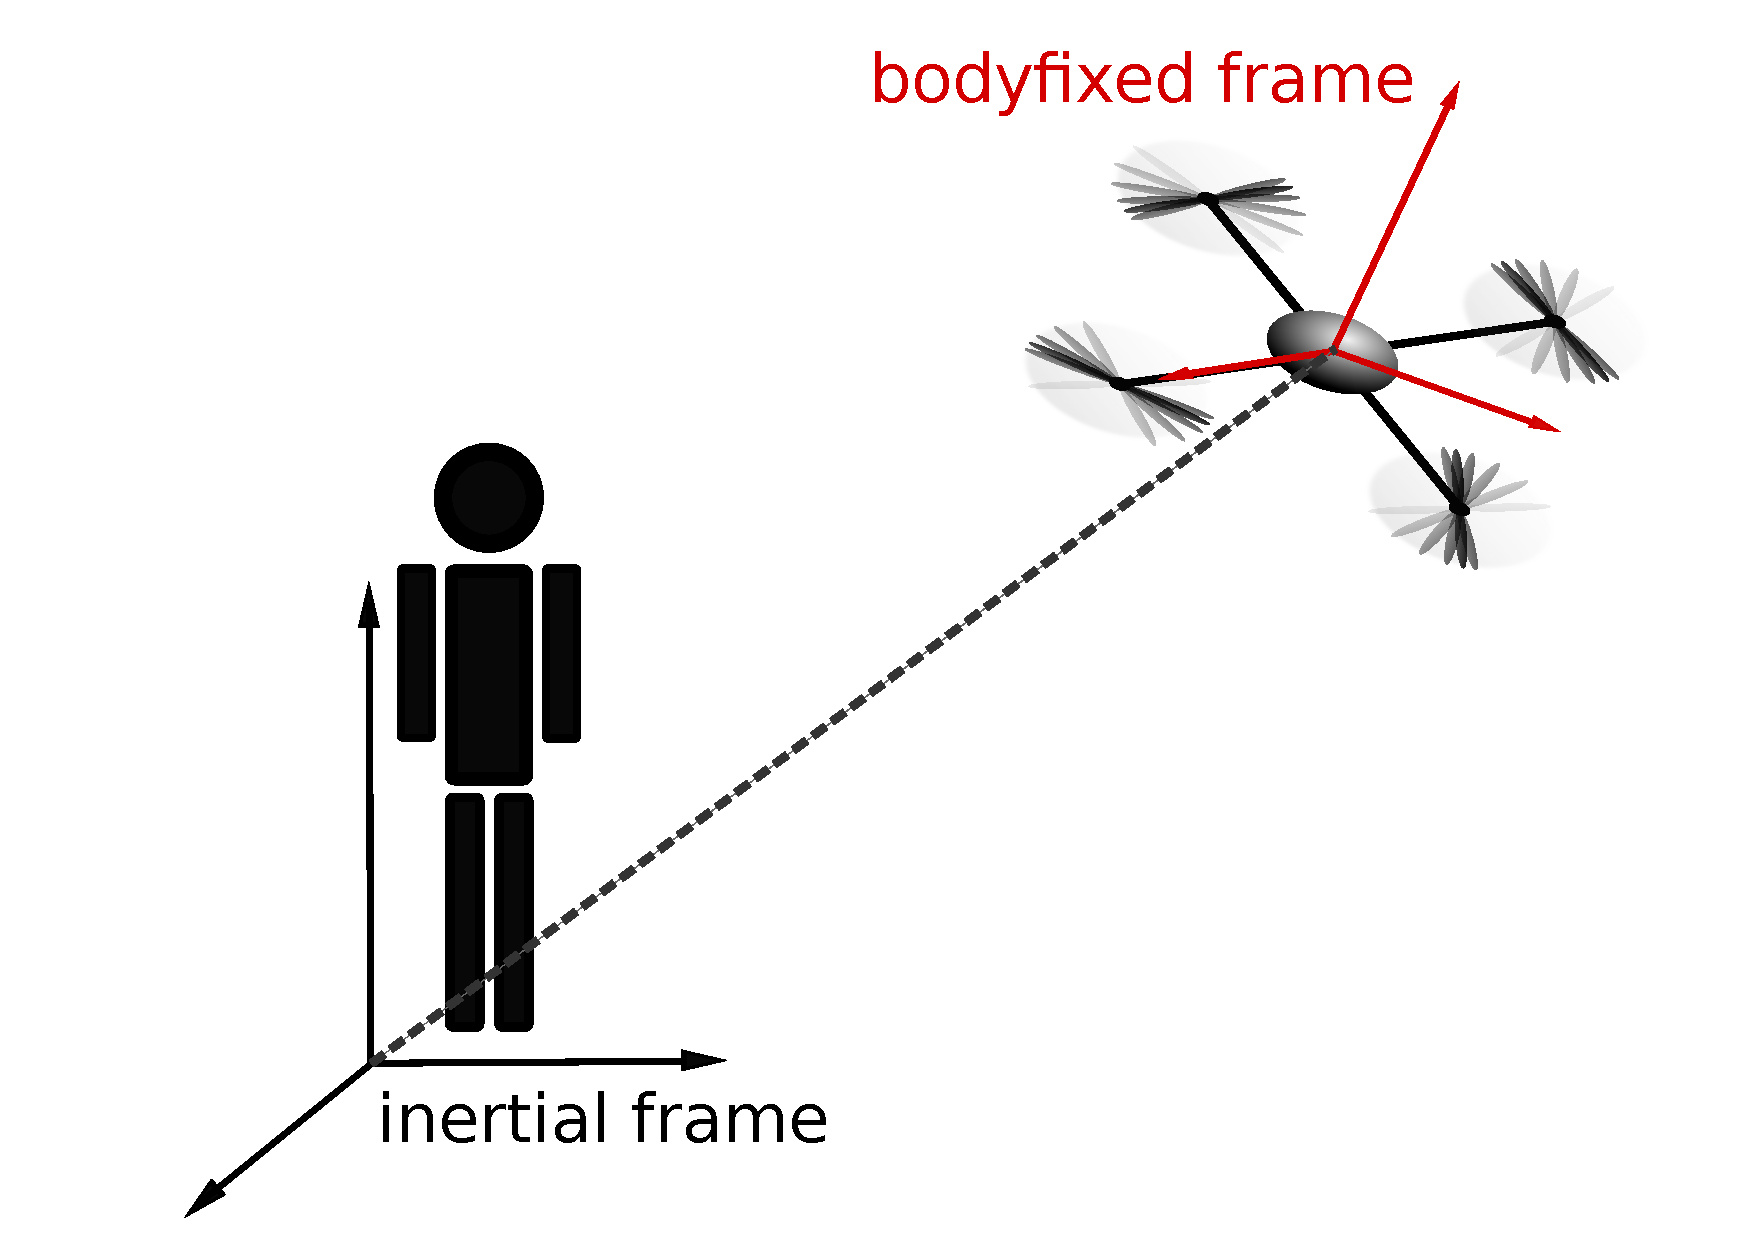
\includegraphics[width=0.8\textwidth]{images/Koordinatensysteme.pdf}
			\label{fig:Koordinatensysteme}
	\end{figure}
\end{frame}

%\begin{frame}
	%\frametitle{Quaternions}
	%\begin{block}{}
		%\centering
		%\vspace{1ex}
		%\( q = a + \textup{i}b+\textup{j}c+\textup{k}d \qquad a, b, c, d \in \mathbb{R} \)
		%\vspace{1ex}
	 %\end{block}
	%\end{frame}

\begin{frame}
	\frametitle{Quaternions}
	\begin{block}{}
		\centering
		\( q = a + \textup{i}b+\textup{j}c+\textup{k}d \qquad a, b, c, d \in \mathbb{R} \) \\
		\vspace{.5ex}
		\(\Leftrightarrow\) \\
		\vspace{1ex}
		\( \hspace{1ex} q = \begin{pmatrix} a \\ b \\ c\\ d \end{pmatrix} \in \mathbb{R}^4 \)
	\end{block}
	
	\vspace{1em}
			\onslide<2-> \centering
			represent rotation \( \quad \Leftrightarrow \quad \Vert q \Vert = 1 \quad \Leftrightarrow \quad q \in \mathcal{S}^3\) 
\end{frame}

\begin{frame}
	\frametitle{Drift Correction}
		\begin{columns}[T] % align columns
			\begin{column}{.55\textwidth}
			\centering
				\begin{textblock}{0}(-4.4,-5)
					\begin{tikzpicture}[scale=4]

	%Colors
	\definecolor{red}{RGB}{190,0,0};
  
  % Styles
  %\tikzstyle{axes}=[->]
	\tikzstyle{every node}=[font=\normalsize]

  % The graphic
  \draw[style=help lines,step=1cm] (-1.2,0) (1.2,1.2);
  \draw[thick] (0,0) (0:1cm) arc (0:98:1cm) ;
    
  \begin{scope}%[style=axes]
    \draw[thick,->] (-.2,0) -- (1.2,0) node[anchor=west] {};
    \draw[thick,->] (0,-.2) -- (0,1.5) node[anchor=west] {};

    \foreach \x/\xtext in {1}
      \draw[xshift=\x cm] (0pt,1pt) -- (0pt,-1pt) node[below,fill=white] {$\xtext$};
		\foreach \y/\ytext in {1}
      \draw[yshift=\y cm] (0pt,1pt) -- (0pt,-1pt) node[left=5pt,fill=white] {$\ytext$};
  \end{scope}
  
  \node at (25:1cm) (q0) [circle, draw, fill=black, inner sep = 0.07cm]{};
	\node[right=3pt] at (25:1cm) {$q_0$};
	\node at (0.5cm,1.294cm) (q1) [circle, draw, fill=black, inner sep = 0.07cm]{};
	\node<1>[right=3pt] at (q1) {$q_1=q_0+\Delta h\cdot \dot{q}_0$};
	\draw<1>[red, thick,->] (q0) to (q1);
	
	\node<2>[right=3pt] at (0.5cm,1.281cm) {$q_1$};
	\draw<2>[thick] (q0) to (q1);
	\node<2> at (68.87:1cm) (q1_normed) [circle, draw, fill=black, inner sep = 0.07cm]{};
	\node<2>[below=5pt] at (68.87:1cm) {$\mathlarger{\frac{q_1}{\|q_1\|}}$};
		\draw<2>[dashed,red,thick,->] (q1) -- (q1_normed) node[anchor=west] {};
\end{tikzpicture}
				\end{textblock}
			\end{column}
			\hfill
			\begin{column}{0.45\textwidth}
				\begin{textblock}{.963\columnwidth}(0,0)
					\begin{block}{}
					\centering
						\( \dot{q}(t) = \tilde{f}(q(t))\only<2->{-\lambda(q(t))} \)
					\end{block}
				\end{textblock}
				\end{column}
		\end{columns}
\end{frame}

%\begin{frame}
	%\frametitle{Drift Correction}
		%\begin{columns}[T] % align columns
			%\begin{column}{.55\textwidth}
				%\begin{textblock}{0}(-4.4,-5)
					%\begin{tikzpicture}[scale=4]

	%Colors
	\definecolor{red}{RGB}{190,0,0};
  
  % Styles
  %\tikzstyle{axes}=[->]
	\tikzstyle{every node}=[font=\normalsize]

  % The graphic
  \draw[style=help lines,step=1cm] (-1.2,0) (1.2,1.2);
  \draw[thick] (0,0) (0:1cm) arc (0:98:1cm) ;
    
  \begin{scope}%[style=axes]
    \draw[thick,->] (-.2,0) -- (1.2,0) node[anchor=west] {};
    \draw[thick,->] (0,-.2) -- (0,1.5) node[anchor=west] {};

    \foreach \x/\xtext in {1}
      \draw[xshift=\x cm] (0pt,1pt) -- (0pt,-1pt) node[below,fill=white] {$\xtext$};
		\foreach \y/\ytext in {1}
      \draw[yshift=\y cm] (0pt,1pt) -- (0pt,-1pt) node[left=5pt,fill=white] {$\ytext$};
  \end{scope}
  
  \node at (25:1cm) (q0) [circle, draw, fill=black, inner sep = 0.07cm]{};
	\node[right=3pt] at (25:1cm) {$q_0$};
	\node at (0.5cm,1.294cm) (q1) [circle, draw, fill=black, inner sep = 0.07cm]{};
	\node[right=3pt] at (0.5cm,1.294cm) {$q_1$};
	\draw[thick] (q0) to (q1);
	\node at (68.87:1cm) (q1_normed) [circle, draw, fill=black, inner sep = 0.07cm]{};
	\node[below=5pt] at (68.87:1cm) {$\mathlarger{\frac{q_1}{\|q_1\|}}$};
	\draw[dashed,red,thick,->] (q1) -- (q1_normed) node[anchor=west] {};
\end{tikzpicture}
				%\end{textblock}
			%\end{column}
			%\hfill
			%\begin{column}{0.45\textwidth}
				%\begin{textblock}{.9\columnwidth}(0,0)
					%\begin{block}{}
					%\centering
					%\( \dot{q}(t) = \tilde{f}(q(t))\only<2->{-\lambda(q(t))} \)
					%\end{block}
				%\end{textblock}
				%\end{column}
		%\end{columns}
%\end{frame}

%TODO:
%  1. Zitate, Quellen (welche Auswahl?) - ok
%  2. Quellen vor oder nach "`Frage"' Seite 
%  3. Mindmap
%  4. passt alles zusammen?
%  5. Quaternionen-Bild - ok
%  6. PS Settin???? andere Überschrift?
% 

\nocite{Boyd2009}
\nocite{Diehl2001}
\nocite{Diehl2002}
\nocite{Diehl2005}
\nocite{Diebel2006}
\nocite{Garcia2013}
%\nocite{Richter-Gebert2009}
%\nocite{Reyes-Valeria2013}
%\nocite{Hartmann2014}
%
\begin{frame}[allowframebreaks] % Literaturverzeichnis über mehrere Frames
 \frametitle{References}
	\bibliography{Literaturliste}
	\bibliographystyle{plain}
\end{frame}
\end{document}
